\documentclass[a4paper,11pt,titlepage]{article}
 
\usepackage[utf8]{inputenc}
\usepackage[spanish]{babel}
\usepackage[T1]{fontenc}
\usepackage{lmodern}
\usepackage{float} %para colocar la imagen en su lugar
 
\usepackage{parskip}
\usepackage{graphicx}
\usepackage{xcolor}
\providecommand{\e}[1]{\ensuremath{\times 10^{#1}}} %Para escribir la notacion cientifica mejor
\definecolor{gris}{RGB}{220,220,220}
 
\begin{document}
\begin{titlepage}
  \vspace*{4cm}
  {\fontsize{28}{34}\selectfont\bfseries Antenas de telefonía móvil}
  \par
  \vspace{0.5cm}
  \centering
  % Logo
  
\includegraphics[height=3cm]{movilportada} \\
  % Línea gris
  \vspace{0.5cm}
  {\color{gris}\hrule}
  \Large{\itshape Radiación y propagación electromagnéticas}
  \vfill
  {\large Manuel de la Cruz González \hfill Abril 2019}
\end{titlepage}
\tableofcontents
\newpage
%EVOLUCION
\section{Evolución de las antenas de teléfonos móviles}
%GEN CERO
\subsection{Generación cero o radio-móvil}
Esta generación recibe el nombre de precelular ya que es anterior a la generación de teléfonos móviles. \par
Los radio-móviles se diferencian de los radioteléfonos (walkie-talkie) en que la tecnología que utilizaban estaba disponible como servicio comercial conectado a la red de telefonía pública, mientras que los walkie talkie y demás sistemas de radioafición son independentes de la red de telefonía.\par
\begin{figure}[H]
\centering
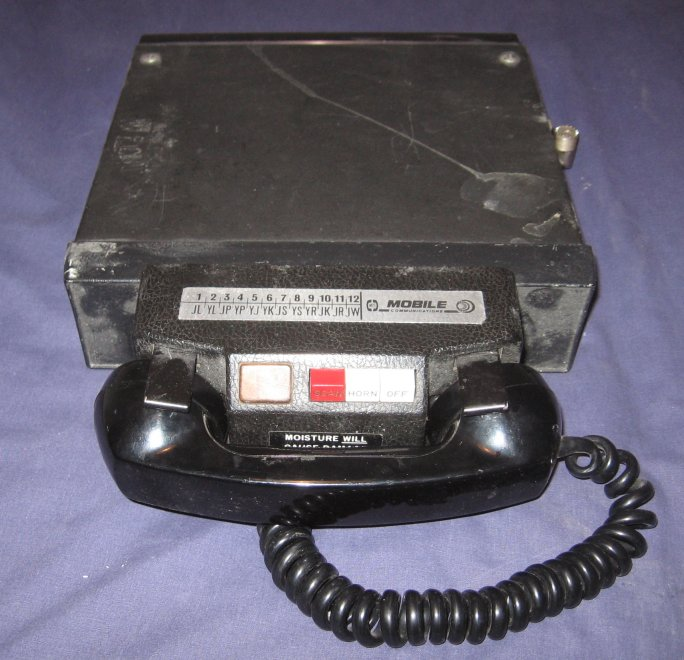
\includegraphics[width=0.5\textwidth]{cero}
\caption{Radio móvil}
\label{imagencero}
\end{figure}
Estos dispositivos se solían utilizar en coches o camiones, llegando a existir en forma de maletín. Las antenas eran externas y estaban situadas en el vehículo donde estaba instalado el radio-móvil.
Este servicio de comunicación comenzó en EEUU en 1946 gracias a la compaía Motorola en unión con Bell System. En Europa comenzaron a usarse en 1952 (República Federal Alemana) y para 1978 (Czechoslovakia) la mayoría de países disponían de este servicio.
%GEN 1
\subsection{Primera Generación o 1G}
Esta generación es la primera de los móviles como los conocemos hoy en día. Esta tecnología analógica comenzó en 1980 y no parói hasta ser sustitutida por el 2G. La principal diferencia entre el 1G y el 2G es que las radio señales que usaban las redes de 1G son analógicas mientras que las de 2G son digitales.\par
La frecuencia de trabajo de estos equipos era de 800 Mhz.
El primer equipo portable de antena para un cuarto de onda tenía una longitud de 9.4 cm y era antena única, no un array.
El primer móvil lanzado al mercado fue el Motorola DynaTAC8000X y la antena que utiliza es una "sleeve dipole". Esta antena no se usa en móviles actuales sin embargo, se usa bastante es dispositivos de comunicación LAN.\par
\begin{figure}[H]
\centering
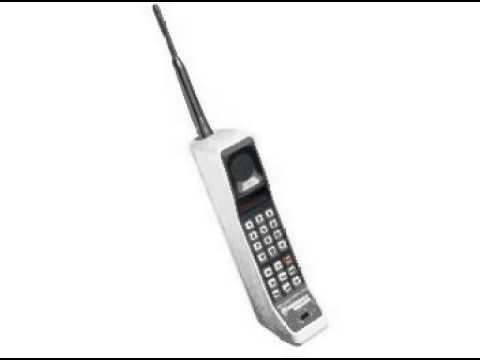
\includegraphics[width=0.6\textwidth]{motorola1}
\caption{Motorola DynaTAC8000X}

\label{motoroladyna}
\end{figure}
Esta antena tiene un consumo eficiente y la longitud se aproximaba a la semilongitud de onda de 850MHz (17 cm).
%GEN 2
\subsection{Segunda Generación o 2G}
En la década de 1990 el 2G trajo varias innovaciones en la telefonía como los servicios de SMS. Se comenzó a operar en GSM 900MHz y más tarde en 1800 MHz.\par
Como ya hemos dicho, su principal diferencia con su predecesora era que ahora este sistema usaba tecnología digital en su network. Esto permitió aumentar la frecuencia y con ello dar más servicios al mismo tiempo.\par
La segunda generación comenzó utilizando únicamente una banda de frecuencia por dispositivo. Así, el Nokia 1011 soportaba sólo GSM900 mientras que otros dispositivos como el Motorola m300 utilizaban GSM1800.\par
Estos teléfono utilizaban dos antenas de monopolo.
\begin{figure}[h]
\centering
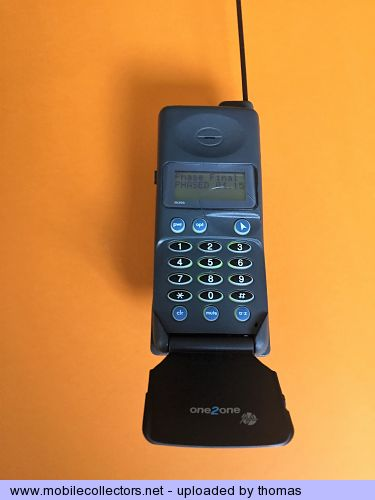
\includegraphics[width=0.6\textwidth]{motorolam300}
\caption{Motorola m300 funcionaba sólo en GSM1800}
\label{motorolam300}
\end{figure}
\par
En 1997, Motorola sacó al mercado el mr601 que fue el primer móvil con dual band. Soportaba tanto GSM1800 como GSM900. Su antena consistía en dos antenas helicoidales cuya forma de onda era de sacacorchos con polarización circular y cuya antena podía ser considerada como tipo dipolo, con patrón de radiación omnidireccional.
\begin{figure}[H]
\centering
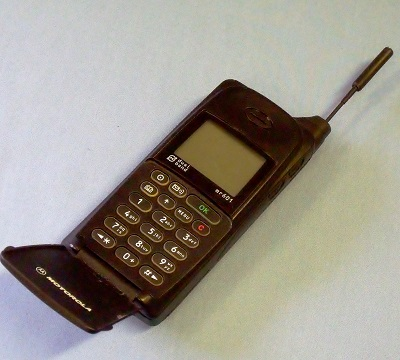
\includegraphics[width=0.6\textwidth]{motorolamr601}
\caption{Motorola mr601}
\label{motorolamr601}
\end{figure}
\par
El siguiente gran avance fueron las antenas tipo PIFA, de las que hablaremos posteriormente. La primera antena PIFA de doble banda operaba a GSM900 y GSM1800 y fue inventada en 1996 por el profesor Peter Hall en U.K.
\par
\begin{figure}[H]
\centering
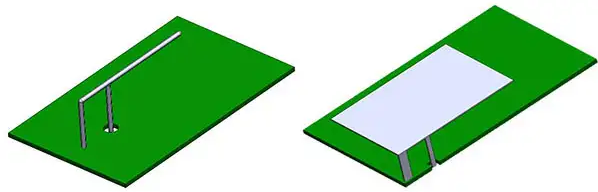
\includegraphics[width=0.6\textwidth]{pifa1}
\caption{Antena planar en forma de T invertida (PIFA)}
\label{pifa1}
\end{figure}
El avance en tecnología móvil se ha sido progresivo. En 1999, Nokia lanza al mercado el primer móvil con antena totalmente interna, soportaba doble banda e hizo 160 millones de ventas.
\begin{figure}[H]
\centering
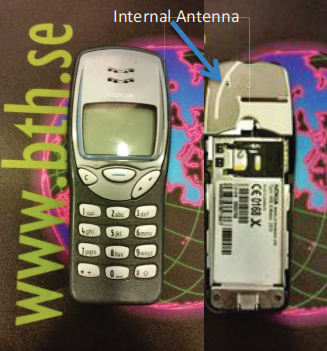
\includegraphics[width=0.6\textwidth]{nokia3210}
\caption{Nokia 3210 y su antena interna}
\label{nokia3210}
\end{figure}

En 1999, el profesor Peter Hall de nuevo, crea la primera PIFA de triple banda que podía operar a 800/1800 y 1900 MHz. Esto marcaría el comienzo de la nueva tecnología 3G.
\newpage
%3 GEN
\subsection{Generaciones posteriores}
La primer red comercial de 3G fue lanzada por Hutchinson Telecommunications en junio de 2003. En 2004 Nokia lanza el modelo Nokia 6630 que fue el primero que permitió el Roaming Global, ya que soportaba GSM 900/1800/1900 y UMTS 2100. En la siguiente imagen podemos ver las antenas de este dispositivo y su localización.
\begin{figure}[H]
\centering
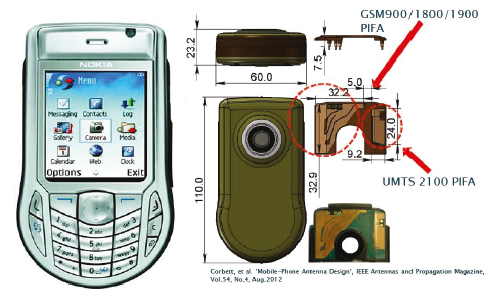
\includegraphics[width=0.7\textwidth]{nokia6630}
\caption{Nokia 6630 y sus antenas}
\end{figure}
A partir de este momento, las antenas móviles evolucionarán en forma de arrays. En la siguiente tabla se expone cronológicamente este desarrollo.
\begin{figure}[H]
\centering
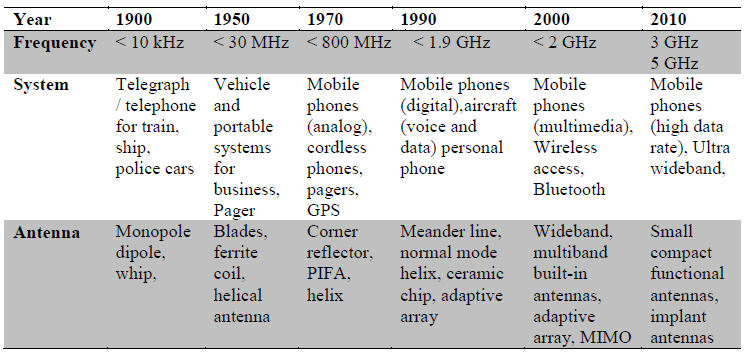
\includegraphics[width=1.2\textwidth]{crono}
\caption{Desarrollo de las antenas}
\end{figure}
Los sistemas de navegación móviles han contribuido al desarrollo del diseño de antenas, mientras que la introducción de nuevos servicios diferentes a una simple llamada ha creado la necesidad de añadir pequeñas antenas también.
El desarrollo de estos arrays ha provocado que antenas como la PIFA hayan sido modificadas tanto que cueste reconocerla de la original. \par
En la década de los 2000 se desarrolla para las comunicaciones la tecnología MIMO.\par
\textbf{MIMO} (Multiple inputs-multiple outputs) es una técnica para enviar y recibir más de una señal de datos al mismo tiempo por un mismo canal mediante la propagación multicamino. Esta técnica aumenta la eficiencia espectral de un sistema de comunicación inalámbrica por medio de la utilización del dominio espacial.
\begin{figure}[H]
\centering
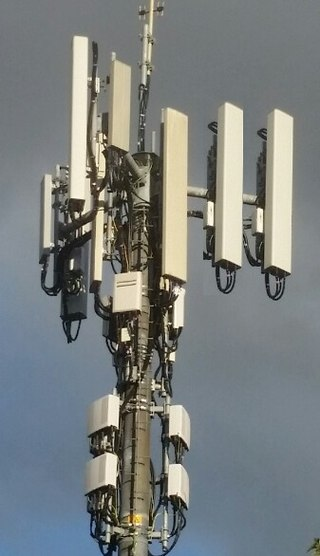
\includegraphics[width=0.4\textwidth]{mimo}
\caption{Antena utilizada para conexiones MIMO}
\end{figure}
Las antenas de los móviles modernos suelen estar directamente impresas en el circuito.\par
\begin{figure}[H]
\centering
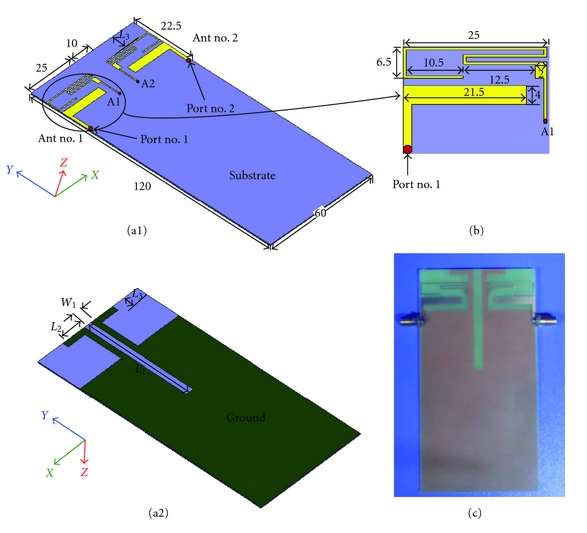
\includegraphics[width=0.95\textwidth]{mimomovil}
\caption{a) y b) Diseño de antena MIMO, c) antena MIMO fabricada}
\end{figure}
El rol de MIMO es fundamental en standards de comunicación inalámbrica como IEE 802.11n (WiFi), HSPA+ (3G), WiMAX (4G), y Long Term Evolution (4G LTE).
%Tipos de antena
\section{Tipos de antena}
\subsection{Antena PIFA}
Es un tipo de antena que consiste en una antena de monopolo que va en paralelo con un plano(ground plane) y está conectada a tierra por un extremo. La antena se alimenta por un punto intermedio a una distancia del extremo conectado a tierra. Tiene ventajas sobre un monopolo simple, la antena es más corta y mucho mas compacta y la impedancia se puede diseñar sin necesidad de añadir nuevos elementos. Fue diseñada en 1950 e implementada con tecnología planar para móviles.
\begin{figure}[H]
\centering
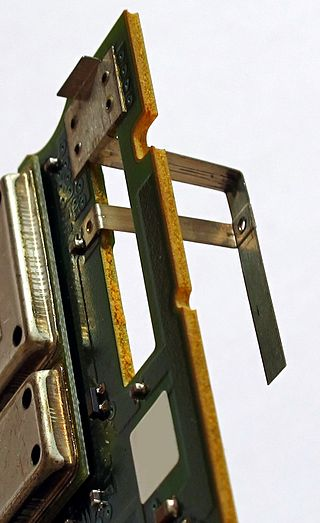
\includegraphics[width=0.25\textwidth]{pifawiki}
\caption{Antena PIFA de una estación}
\end{figure}
La PIFA puede ser utilizada en dispositivos móviles al ser implementada en un microstrip. En el microstrip también puede haber filtros integrados y demás dispositivos para mejorar la comunicación.\par
La implementación puede ser en la forma de PIFA clásica, desplazando el plano de tierra; o bien como antena de parche (patch antenna). En la patch antenna, al borde del patch se unen a tierra varios pins que van hacia el plano de tierra. El concepto de antena en F es el mismo, pero ahora la antena tiene más ancho de banda al tener más área de radiación. 
\begin{figure}[H]
\centering
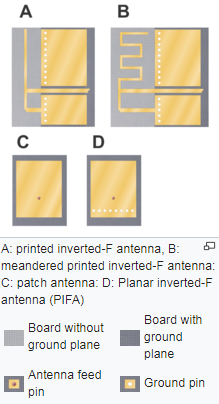
\includegraphics[width=0.4\textwidth]{pifaplanar}
\end{figure}
Las principales ventajas de las PIFA son:
\begin{itemize}
\item[+] Pequeño tamaño con la tecnología planar.
\item[+] Alta ganancia para polarización horizontal y vertical.
\item[+] Coste bajo.
\item[+] "Backward radiation" baja, por lo que afectan poco a la salud.
\end{itemize}
Su principal problema es la sensibilidad, pero esta puede ser mejorada mediante métodos como MIMO.
%Antena fractal
\subsection{Antena fractal}
Las antenas fractales utilizan un diseño fractal diseñado para maximizar la superficie de recepción de una señal. Estas antenas solucionan el problema de que las antenas convencionales operan en un ancho de banda muy estrecho, mientras que las fractales aumentan este ancho de banda de trabajo de manera considerable.\par
También es digno de mención que experimentos con estas antenas han demostrado un mejor rendimiento para longitudes de cuarto de onda que las antenas convencionales.
\begin{figure}[H]
\centering
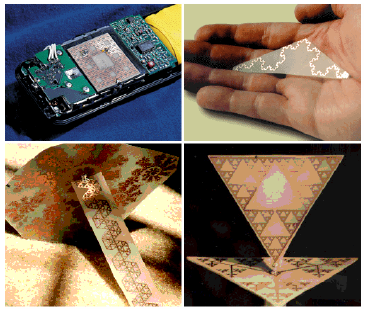
\includegraphics[width=0.6\textwidth]{fractal}
\caption{Antenas fractales triangulares. Arriba izda: Patch Antenna Fractal. Arriba dcha: Fractal triangular. Abajo izda: Monopolo fractal. Abajo dcha: Bowtie Monopolo Fractal. }
\end{figure}
\section{Diseño de una antena de GPS}
La antena de GPS es omnidireccional y sólo tiene modo de recepción. La frecuencia del GPS es de 1.575 GHz, sin prácticamente ancho de banda.\par
Los satelites de GPS envían señales polarizadas circularmente, en concreto utilizan RHCP (Right Hand Circular Polarization). Esto es beneficioso ya que no necesitamos alinear nuestra antena en el eje de rotación.\par 
El problema principal de la señal de GPS es que su densidad en potencia es muy baja cuando llega a la Tierra. Encontramos niveles de hasta -160dB, por lo tanto; necesitamos una antena eficiente para el receptor. A continuación mostramos un móvil en el que se muestra la localización de esta antena y sus características:
\begin{figure}[H]
\centering
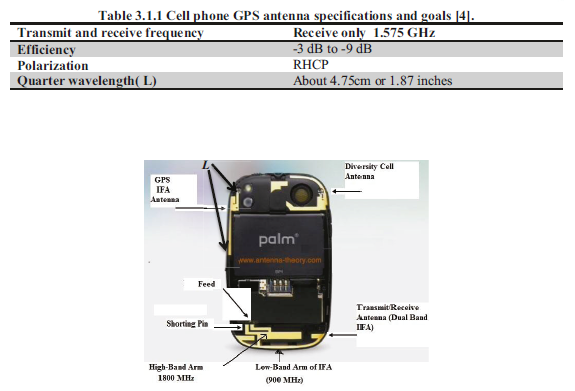
\includegraphics[width=1.1\textwidth]{movilgps}
\caption{Características típicas de GPS de un móvil y su localización}
\end{figure}
Como vemos en la imagen, la antena de GPS está localizada en la parte superior del dispositivo para garantizar su mejor funcionamiento. Esto es también porque por lo general, los usuarios toman verticalmente el móvil cuando quieren recibir una señal GPS, por tanto sus manos se encuentran alejadas de la antena. También el GPS está situado en un lugar compatible con el buen funcionamiento del resto de antenas.\par 
Para obtener una antena de dipolo con polarización circular, usamos dos dipolos cruzados para dar las dos componentes ortogonales al campo. Esto hace que a lo largo del zenit, si los dipolos se alimentan con un desfase de 90º, la polarización sea circular.
\section{Diseño de una antena PIFA de una sola frecuencia}
La construcción típica de esta antena se hace sobre un bloque de nylon que separa el dibujo de la antena del plano de tierra.
\begin{figure}[H]
\centering
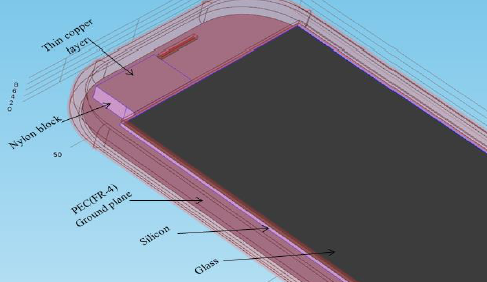
\includegraphics[width=0.7\textwidth]{pifanylon}
\caption{Esquema de construcción}
\end{figure}
Si queremos construir una antena de 1.575 GHz como frecuencia resonante y una ganancia entre -3dB (caída de 50\% de potencia) y 0 dB el diseño geométrico será de la forma:
\begin{figure}[H]
\centering
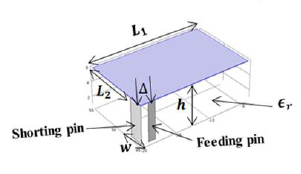
\includegraphics[width=0.8\textwidth]{esquemapifa}
\end{figure}
\newpage
La frecuencia resonante puede ser calculada de la siguiente forma:\par
$$ L_1+L_2-W=\frac{\lambda_0}{4}$$
Mientras que la relación entre la longitud de onda resonante y la frecuencia es:
$$ \lambda_0=\frac{c_0}{f_0\sqrt{\epsilon_r}}$$
Podemos ver que la antena puede reducirse en tamaño al aumentar la permitividad relativa pero también afecta a la ganancia de la antena.Valores típicos de esta antena serían:
$$L_1=20mm, L_2=10mm, W=2mm, h=4mm, \epsilon_r=3.8$$
Con esto obtendría:
$$20+10-2=\frac{\lambda_0}{4}, \lambda_0=112mm$$
$$f_0=\frac{3\times 10^{8}}{112\times 10^{-3}\sqrt{3.8}}=1.374 GHz$$
Que es una frecuencia de resonancia cercana a la propuesta.
A continuación, presentamos una tabla de materiales con sus constantes dieléctricas.
\begin{figure}[H]
\centering
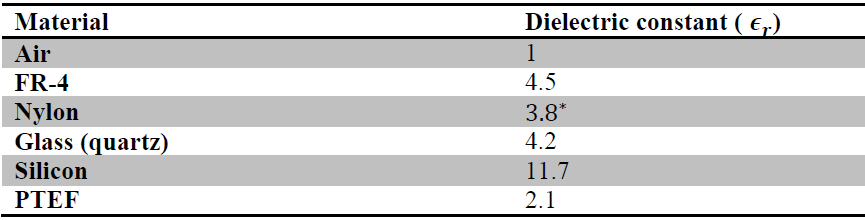
\includegraphics[width=0.8\textwidth]{materiales}
\end{figure}
Mediante un programa de simulación (COMSOL) se puede observar el patrón de ganancia de la antena PIFA de una sola frecuencia en el plano xy.
\begin{figure}[H]
\centering
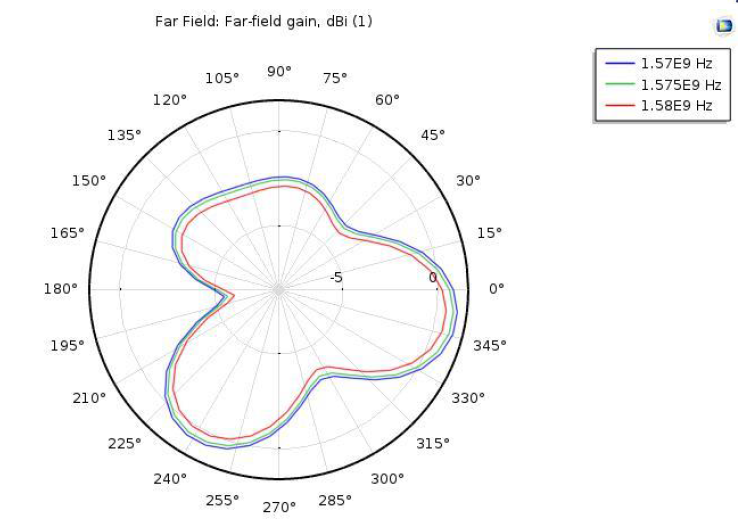
\includegraphics[width=0.8\textwidth]{ganancia}
\end{figure}
Podemos observar que esta antena relativamente omnidireccional, aunque existen direcciones privilegiadas en 0º, 120º y 240º.
\section{Diseño de una antena PIFA de banda ancha}
En los móviles modernos debido al roaming, las diferentes teleoperadoras actuando a diferentes frecuencias y el aumento de servicios demandados por los consumidores, son necesarias las antenas PIFA multifrecuencia.A una antena PIFA estándar y que use la técnica de la ranura (como vemos en la imagen) se le demanda que se operativa en frecuencias entre 1800 MHz y 2600 MHz. Esto es debido a que los distintos servicios móviles operan a:\par
\begin{itemize}
\item[+] Rango de covertura GSM, estándar europeo de 2G: Entre 1800 y 1900 MHz.
\item[+] UMTS, tecnología 3G basada en GSM (2100 MHz).
\item[+] Bluetooth y WiFi (2.4 GHz).
\item[+] Sistema LTE, asociado a 3G y 4G. (2.3 GHz,2.5 GHz y 2.6 GHz)
\end{itemize}
\begin{figure}[H]
\centering
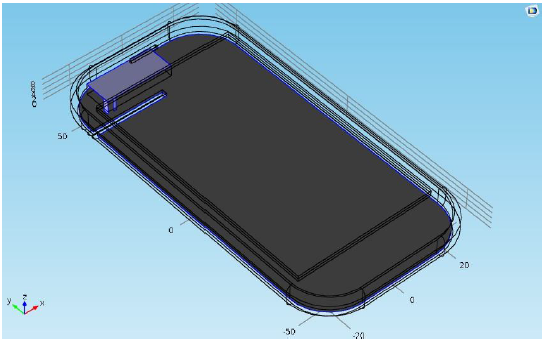
\includegraphics[width=0.8\textwidth]{pifamulti}
\caption{Antena PIFA de ranura.}
\end{figure}
Veamos ahora el esquema de la antena, los valores típicos que toman sus parámetros y la frecuencia y ancho de banda que abarca la antena. La fórmula es la misma para calcular la frecuencia que para la PIFA de una sola frecuencia. \par
Para los valores de:
\begin{itemize}
\item[+] $L_1=24mm$, $L_2=10mm$, $h=4mm$, $W=2mm$
\item[+] $d_s=5mm$, $L_S=28mm$ y $W_S=2mm$
\end{itemize}

\begin{figure}[H]
\centering
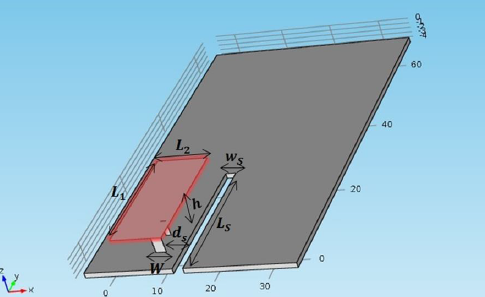
\includegraphics[width=0.8\textwidth]{parametrosmulti}
\end{figure}
Obtengo: \par
$$f_0=\frac{3\times 10^{8}}{128 \times 10^{-3}\sqrt{1}}=2.343 GHz$$
\par
Mediante el programa de ordenador se obtiene que para esos parámetro el ancho de banda es de un 36\% respecto a la frecuencia central de 2.200 MHz. Si el ancho de banda es superior al 20\% se considera banda ancha.


%FIN
\end{document}
